%!TEX TS-program = xelatex
%!TEX encoding = UTF-8 Unicode

\documentclass{../../../lib/gs}

% Configurazione per URL su nuova linea
\DeclareFieldFormat{url}{\newline\footnotesize\url{#1}}
\DeclareFieldFormat{howpublished}{\newline\footnotesize#1}
\DeclareFieldFormat{urldate}{\mkbibparens{#1}}

\usepackage{../../../lib/apf}
\newfontfamily\phonfont{Charis} % font ricco di simboli IPA

% Packages per figure e grafici
\usepackage{pgfplots}
\pgfplotsset{compat=1.18}
\usepackage{tikz}
\usetikzlibrary{decorations.text}
\usepackage{subcaption}

\usepackage{enumitem}

\title{come un filtro AllPass}
\subtitle{autobiografia di un eretico. appunti revb.}
\author{Giuseppe Silvi}
\date{\today}

% Definizione delle parole chiave per i metadati PDF
\kuno{filosofia}
\kdue{greco antico}
\ktre{Platone}
\kquattro{etimologia}
\kcinque{XeLaTeX}

% Comandi per la notazione AllPass
\newcommand{\apf}[3]{\textbf{\texttt{#1(#2,#3)}}}
\newcommand{\apfc}[3]{\begin{center}\apf{#1}{#2}{#3}\end{center}}
\newcommand{\apfcn}[4]{\begin{center}\apf{#1}{#2}{#3}\footnote{#4}\end{center}}

% Nel preambolo del .tex
\addbibresource{../../bibliografia.bib}

\begin{document}

\maketitle

C'è una sola parola d'ordine per comprendere, decifrare le motivazioni, ciò che
mette in movimento questo tentativo di assedio attorno all'esperienza musicale,
questa ossessione per i legami tra «parole alate», per i ponti tra processi
differenti che d'istinto vivo come un labirinto donato da antichissime umanità e
che, semplicemente, chiamo musica: \emph{risonanza}. «Se c’è una parola che ne
indichi la poetica è risonanza.» \cite{netti24}

\begin{quote}
  \begin{sf}
    \small
    Il presente, l'\emph{Anwesend}, deve avermi già rivolto la parola nel suo
    essere presente. \cite{agamben19}
  \end{sf}
\end{quote}

Cosa di me risuona a questo presente? Che parte del mio me risuona? Dove risuona?
Che cos'è questa risonanza se non un ri-sentire, un aver risentito fisicamente
dell'impronta del presente e anche un aver ri-sentito altrove ciò che ormai non
è più, perché passato? Tra-passato da ciò che si sta eternamente allontanando da
me io ri-suono. \cite{ronchi2001}

{\phonfont su̯en-}\footnote{Pokorny IEW 1046-47: to sound, resound.} $ \rightarrow $
suono $ \rightarrow $ \emph{ri-}, di nuovo, \emph{-suono}, suono di nuovo. È
ciò che oggi mi mette in risonanza con l'età del rame: {\phonfont su̯en-} la radicalità
della risonanza in quattro lettere in altrettanti migliaia di anni.

I perché come e dove sono le attitudini po-etiche di cui scrive Netti \cite{netti24}
sono le leve che predispongono l'intuizione che muove.

Su \emph{resonantia} c'è poco da aggiungere: \emph{re-} (indietro, di nuovo,
ancora una volta), di nuovo suono in \emph{resonant} che con \emph{-ia} forma
un nome astratto. La risonanza è un nome astratto. È un nome “tratto via”,
“separato da”, \emph{abstractus} da cosa?

Risolvere questi enigmi richiede una pratica della risonanza. Una teoria della
risonanza può aiutare a venirne fuori, a «far luce» \cite{ronchi2001} sulla
faccenda. Una po-etica della risonanza così come la intende Netti\footnote{
  Ho avuto il dono della risonanza da Giorgio Netti nel 2016. Quando decisi di
  studiare la risonanza attraverso lo studio del riverbero era ormai il 2018.
  Era solo il primo colpo tornato in dietro.
} \cite{netti24}
è una necessità.

Quando quel risuonare è stabilito con rapporti molti a molti lo chiamiamo
\emph{riverbero}\footnote{
  Riverbero deriva direttamente dal latino classico \emph{reverberāre}, composto
  dal prefisso \emph{re-} ("indietro, di nuovo") e \emph{verberāre} ("battere,
  colpire"). La radice \emph{verberāre} deriva da \emph{verber, verberis} ("frusta,
  sferza, colpo"), collegandosi infine alla radice protoindoeuropea \emph{wer-}
  che significa "girare, piegare."

  Il significato latino si concentrava su "ripercuotere" - colpire indietro o
  causare un rimbalzo - tuttavia, durante il Rinascimento e il XVIII secolo,
  emersero prominentemente applicazioni tecniche. \emph{Forni a riverbero} (forni
  riverberatori) diventarono cruciali nella metallurgia per processare rame,
  stagno e acciaio usando il riscaldamento radiante. Più significativi
  culturalmente erano i \emph{riverberi pubblici} - sistemi di illuminazione
  stradale precoce che usavano superfici riflettenti per amplificare la luce delle
  lampade a olio, documentati nelle città italiane da Venezia (1732) a Milano
  (1786) a Bologna (1801).
}. Il riverbero (di cui il “ripercuotere” è l'immagine antica) è
una parola tecnica, è l'ambiente fisico della risonanza astratta.

Ma per comprendere come la risonanza si manifesti tecnicamente, dobbiamo prima chiarire cosa sia veramente un filtro - dispositivo che, come vedremo, condivide con la risonanza la necessità di un'intenzionalità progettuale.

\section{che cos'è un filtro?}

La scelta del termine “filtro” per dispositivi elettrici, audio e video è
attribuibile principalmente a George Ashley Campbell dell'\emph{AT\&T}, che nel
1915 introdusse l'espressione “electric wave-filter” nella letteratura scientifica.
Campbell depositò il brevetto fondamentale\footnote{US Patent No. 1,227,113 - 15
luglio 1915, rilasciato il 22 maggio 1917} descrivendo il primo “Electric
Wave-Filter”. Nel 1922 pubblicò l'articolo seminale “Physical theory of the
electric wave-filter” nel \emph{Bell System Technical Journal}, che definì
teoricamente questo nuovo campo. La scelta terminologica non fu casuale:
Campbell stava sviluppando dispositivi che permettevano la trasmissione
attraverso un sistema di una banda di onde tra limiti definiti di frequenza e
discriminavano nettamente frequenze fuori banda.

\begin{quote}
  \begin{sf}
    \small
    Any medium through which the music signal passes, whatever its form, can be
    regarded as a filter. [\ldots] A well-known signal processing wizard is said
    to have remarked, “When you think about it, everything is a filter.”\footnote{
    “Introduction to Digital Filters with Audio Applications”, by Julius O.
    Smith III, (September 2007 Edition)
    \url{https://ccrma.stanford.edu/~jos/filters/What_Filter.html}
    }
  \end{sf}
\end{quote}

Ma se tutto è un filtro, allora nulla più è veramente un filtro - il concetto
perde il suo potere discriminante. Poniamo l'attenzione all'identità matematica
$y(t)=x(t)$. Un'identità non è un filtro: è un'identità. Un oggetto descrivibile
con quella funzione può essere un cavo avente un'entrata e un'uscita. Tuttavia
il circuito precedente potrebbe essere descritto con la funzione di
trasferimento $H(\omega)=1$ per tutte le frequenze, formula che descrive anche
un filtro \emph{AllPass}.

Da un punto di vista fisico, ogni sistema reale introduce qualche alterazione,
più che dire che tutto è filtro, in senso fisico dovremmo partire da “tutto
modifica il segnale”. Un'identità matematica, nel mondo fisico può essere
analizzata e descritta con la stessa matematica di un filtro, pur non essendo un
filtro.

Questa distinzione suggerisce di distinguere tra \emph{filtro} (oggetto o
dispositivo) e \emph{filtraggio} (processo). Un cavo coassiale lungo, per
esempio, subisce un processo di filtraggio a causa delle sue proprietà fisiche
distribuite—resistenza, capacità e induttanza—che attenuano naturalmente le
alte frequenze. Tuttavia il cavo non è un filtro: è stato progettato per
trasportare il segnale il più fedelmente possibile, e l'attenuazione
frequenziale è un effetto parassita indesiderato. Il processo di filtraggio
può avvenire ovunque ci sia selezione frequenziale, ma il filtro come oggetto
richiede intenzionalità progettuale.

In generale la parola filtro \emph{deve funzionare} a prescindere dal campo
fisico. Filtro deriva dal latino \emph{filtrum}, che indicava originariamente un
pezzo di feltro (\emph{feltrum}) usato per filtrare i liquidi. Un filtro può
avere luogo solo con una radicale intenzionalità: \emph{filtrum} implica
intenzionalità di separazione. Anche una persona ha entrata (udito) e uscita
(voce) e, in una discussione, filtra il discorso solo se vuole farlo. Altrimenti,
si dice che perde parti del discorso, che dimentica cose o, al limite, che le inventa\ldots
Quando qualcuno filtra intenzionalmente: seleziona, omette, riorganizza il
discorso per un obiettivo; quando qualcuno altera non intenzionalmente:
dimentica, confonde, inventa. Sono due categorie ontologicamente diverse. Nel
secondo caso non diciamo che “filtra male” - diciamo che ha problemi di memoria,
attenzione, o comprensione.

\begin{quote}
  \begin{sf}
    \small
    The different vowel sounds in speech are produced primarily by changing the
    shape of the mouth cavity, which changes the resonances and hence the
    filtering characteristics of the vocal tract.\footnote{
    “Introduction to Digital Filters with Audio Applications”, by Julius O.
    Smith III, (September 2007 Edition)
    \url{https://ccrma.stanford.edu/~jos/filters/What_Filter.html}
    }
  \end{sf}
\end{quote}

La risonanza non è un filtro, tuttavia un filtro può portare alla risonanza: la
cavità orale non “filtra” di per sé - semplicemente ha proprietà risonanti. Il
filtraggio avviene quando il parlante modula consapevolmente quelle proprietà
per produrre suoni specifici. È l'intenzionalità che trasforma una cavità
risonante in un filtro vocale.

Il concetto di filtro ha una dimensione teleologica essenziale: richiede
l'intenzione di separare, selezionare, trattenere. Tutto è filtro può portare a
un errore categoriale, confondendo causalità fisica con intenzionalità
progettuale, svuotando così il concetto del suo significato operativo.

\section{qualcosa appare a partire da se stesso: \emph{come un allpass}}

\begin{quote}
  \begin{sf}
    \small
    In che senso si può dire dell'\emph{Anwesend} che in esso comune è da dove
    io parto e dove arrivo? Eraclito l'aveva mostrato per il cerchio, Parmenide
    per la sfera. Ma come pensarlo senza ricorrere all'immagine del cerchio?
  \end{sf}
\end{quote}

Posso pensarlo come circuito. Posso pensarlo come un filtro \emph{AllPass}. In
un diagramma che rappresenti il circuito del filtro \emph{AllPass} il cerchio è
una proiezione del suo doppio movimento.

\begin{figure}[ht]
  \centering
  \begin{tikzpicture}
    \tikzstyle{every node}=[font=\small]
    \ciclodiagram{}{}{}
  \end{tikzpicture}
  %\includegraphics{tikz/ciclo-base/ciclobase.pdf}
  %\captionsetup{width=.81\linewidth}
  %\caption{}
  \label{tikz:ciclobase}
\end{figure}



\begin{figure}[ht]
  \centering
  \begin{tikzpicture}
    \tikzstyle{every node}=[font=\small]
    \ciclodiagram{t=sè stesso}{}{}
  \end{tikzpicture}
  %\includegraphics{tikz/ciclo-base/ciclobase.pdf}
  %\captionsetup{width=.81\linewidth}
  %\caption{}
  \label{tikz:ciclobase}
\end{figure}

Consideriamo quindi l'essere in funzione della sua memoria (oppure la funzione
memoria dell'essere), il presente, l'\emph{Anwesend}, è un segnale esterno.
L'\emph{Anwesend}, \emph{signāle}, un “qualcosa che serve da segno”. È un
\emph{*sekw-}, seguire qualcosa «nel suo essere presente» che lascia un segno,
«che deve avermi già rivolto la parola».

Caratteristica del filtro \emph{AllPass} è che il presente che si presenta viene
visto, sentito, riflesso. Un segnale che riflette, che rimbalza nell'essere,
lascia una copia, un negativo: una copia inversa e forse un po' sbiadita,
attenuata, del suo passaggio.

Il passare passando, la copia passante di questo passare passando, sfugge. È
puro movimento, allontanamento.

L'essere memoria osserva l'allontanamento, trattiene il passaggio di qualcosa
che sempre si allontana.

\begin{quote}
  \begin{sf}
    \small
    Il logos in quanto enunciazione presuppone, cioè, il \emph{phainōmenon}. In
    questo senso, l'enunciato non è che il dispiegamento o il rivelarsi
    ()\emph{entfaltung}) del fenomeno.
  \end{sf}
\end{quote}

Il fenomeno è l'allontanamento. Il logos, l'enunciazione è il passaggio del
fenomeno per $t=memoria$. «In questo senso, l'enunciato non è che il
dispiegamento.»

Non resta che chiudere il circuito: la copia negativa si somma al logos.
«Rappresentazione e oggetto sono correlativi», \emph{xynon}, una distanza,
una differenza, «il logos è ciò che lascia apparire la coappartenenza di tutte
le cose.»

Questa \emph{physis} designa «l'apparire nella presenza» e questo apparire si
sdoppia in un nuovo doppio movimento: una parte che appare per scomparire per
sempre, in un eterno allontanamento dalla sua apparizione; una parte torna al
suo punto di partenza, in un movimento di riavvicinamento, qualcuno direbbe di
assedio della memoria, qualcuno direbbe che torna ossessione: «che, nella mia
vita, che pure si appresta alla fine, non ha ancora cessato di avvenire.»

\begin{quote}
  \begin{sf}
    \small
    Si tratta, qui, di un sentiero che\ldots apre su se stesso e apre su
    qualcosa. Sentiero nel senso greco di qualcosa che apre, apertura. L'uomo
    moderno non cammina più su un sentiero, ma su una carta geografica.
  \end{sf}
\end{quote}

Un sentiero che apre su se stesso e su qualcosa. Un segnale-sentiero, un sentiero
del segno: una materializzazione della comunicazione nel corto-circuito tra
intenzione e ricezione.

\begin{quote}
  \begin{sf}
    \small
    Il logos è ciò che lascia apparire la coappartenenza di tutte le cose.
  \end{sf}
\end{quote}

La caratteristica prima di questo circuito è che, apparentemente, ciò che lo
attravrsa appare immutato (il segnale in entrata e quello in uscita appaiono
medesimi). Tuttavia, il fenomeno coappartenente al logos non è la stessa cosa.
La costruzione della risonanza (mediante il filtro) si protrae oltre
l'avvenuto\ldots «costruire significa porre insieme», ciò che si
coappartiene\ldots questo «porre insieme» ha il carattere della \emph{thesis},
è, in questo senso, una sin-thesi: e tale è il significato della parola «sistema».

%-------------------------------------------------------------------------------
%----------------------------------------------------------------- SUB-SECTION -
%-------------------------------------------------------------------------------

\subsection{come un filtro \emph{AllPass}}

Questa ricerca si fonda sull'assunto che un linguaggio costituisce un segnale — non un segnale naturale come le posizioni stellari o i cicli giorno-notte, ma un segnale artificiale, basato su principi e modulazioni della materia. A partire da questo fondamento, lo studio propone il filtro \emph{AllPass} come ponte epistemologico tra postura scientifica ed esplorazione artistica, dimostrando come l'elaborazione del segnale (il linguaggio) possa illuminare la natura temporale dell'esperienza musicale senza ridurla ad analisi parametrica.

Il quadro teorico presenta una proprietà ricorsiva: la teoria \emph{AllPass} stessa opera come un filtro \emph{AllPass}

\apfc{APT}{scientifico}{artistico}

\noindent mentre la sua metodologia emerge come

\apfc{metodologia}{postura}{esplorazione}

rivelando una teoria capace di descrivere la propria natura interdisciplinare attraverso la sua stessa notazione fondamentale.

Così come un filtro \emph{AllPass} preserva le energie di un segnale alterandone solo le relazioni temporali, ogni esperienza musicale conserva il contenuto informazionale trasformando continuamente il significato attraverso l'intreccio di materia e memoria. Questo isomorfismo consente una forma di indagine estesa tra tradizioni provenienti dalla cibernetica, teoria dei segnali e l'analisi fenomenologica mantenendo il rigore scientifico e la ricchezza esperienziale.

Ogni formalizzazione dell'esperienza musicale si confronta con questioni epistemologiche fondamentali: \textit{è possibile sviluppare modelli formali che non riducano l'esperienza musicale a combinazioni di parametri fisici? Si può preservare senso in una notazione formale estremamente concisa? Come trasformano, gli strumenti scientifici, la nostra comprensione dei processi creativi?} Il paradigma \emph{AllPass} dimostra che l'opposizione percepita tra analisi scientifica e intuizione artistica si dissolve quando entrambe operano all'interno di domini temporali condivisi.

Questa teoria ha origini nello studio dell'\apf{esperienza}{materia}{memoria} (\cite{bergson1896} - fig. \ref{esperienza}) come elemento necessario e fondante di un pensiero musicale, il cui grado di libertà è in funzione della \apf{creatività}{potenza}{potenza-di-non} (\cite{agamben17}) e la parola è agente performativo dello stupore (\cite{ronchi2001}); questi termini \emph{operano} in funzioni attive e l'isomorfismo del modello \emph{AllPass} consente di mettere in relazione sensi opposti, preservando l'energia dell'informazione e modificandone il comportamento temporale. La cibernetica di secondo ordine (\cite{vonfoerster1981}) fornisce il quadro epistemologico per questo approccio.

La metodologia opera attraverso quattro livelli correlati che emergono dal processo:
\begin{enumerate}[nosep]
  \item analisi filosofica della costituzione temporale e della potenzialità creativa;
  \item rappresentazione circuitale attraverso diagrammi che visualizzano il flusso temporale dei processi (fig. \ref{apf});
  \item notazione formale mediante il sistema simbolico
    \apfc{processo}{fir}{iir}
    che sintetizza relazioni temporali complesse;
  \item implementazione numerica attraverso funzioni di trasferimento (eq. \ref{transfer}) ed equazioni alle differenze discrete (eq. \ref{difference}) che rivelano come relazioni filosofiche tradizionalmente dialettiche divengano complementari in dinamiche processuali, estendendo l'analisi computazionale nel dominio temporale dell'esperienza musicale.
\end{enumerate}

\begin{figure}[htbp]
\begin{center}
\begin{tikzpicture}
  \tikzstyle{every node}=[font=\small]
  \ciclodiagram{processo}{fir}{iir}
\end{tikzpicture}
\caption{Schema del modello AllPass: il processo centrale consiste nell'elaborazione temporale, mentre elementi anticipatori (FIR) precedono l'elaborazione ed elementi ricorsivi (IIR) la seguono, creando una tendenza a feedback infinito. Questo isomorfismo strutturale consente di modellare processi filosofico-musicali complessi nel bilanciamento energetico tra mediazione e immediatezza.}
\label{apf}
\end{center}
\end{figure}

Applicazioni pratiche emergono dall'attuale ricerca elettroacustica presso il LEAP (Laboratorio ElettroAcustico Permanente, Roma), dove il modello consente di analizzare processi critici quali \apf{ascolto}{percezione}{conoscenza} (\cite{diScipio2003}) e relazioni complesse come \apf{artista}{operazione}{opera} in cui ciascun membro può essere decomposto, come nel caso dell'opera stessa in \apf{opera}{strumento}{interprete}, dando forma a reti di filtri di ordini superiori.

Dimostrando come il formalismo circuitale possa potenziare la comprensione artistica, questo lavoro contribuisce a una teoria dell'esperienza musicale computazionalmente e filosoficamente informata che estende il rigore analitico nel dominio temporale proprio del pensiero musicale che si fa esperienza.

% \vspace{1cm}
%
% % PAROLE CHIAVE
% \noindent \textbf{Parole chiave:} fenomenologia, isomorfismo, elaborazione segnale , ricorsività, cibernetica

%\clearpage

%-------------------------------------------------------------------------------
%----------------------------------------------------------------- SUB-SECTION -
%-------------------------------------------------------------------------------

%\subsection*{Figure}



\begin{figure}[htbp]
  \centering
  \begin{subfigure}[b]{0.48\textwidth}
    \centering
    \begin{tikzpicture}
      \tikzstyle{every node}=[font=\small]
      \ciclodiagram{esperienza}{materia}{memoria}
    \end{tikzpicture}
    \caption{Esperienza bergsoniana: la materia come input diretto (FIR) si combina con la memoria ricorsiva (IIR) nel processo dell'esperienza cosciente.}
    \label{esperienza}
  \end{subfigure}
  \hfill
  \begin{subfigure}[b]{0.48\textwidth}
    \centering
    \begin{tikzpicture}
      \tikzstyle{every node}=[font=\small]
      \ciclodiagram{creatività}{potenza}{potenza-di-non}
    \end{tikzpicture}
    \caption{Creatività in Agamben: la potenza attiva (FIR) interagisce con la potenza-di-non (IIR) generando il processo creativo attraverso feedback dialettico.}
    \label{creativita}
  \end{subfigure}
  \caption{Applicazioni del modello AllPass a concetti filosofici fondamentali. (a) La materia come presentazione immediata (FIR) e la memoria come ritenzione e riattualizzazione (IIR). (b) La creatività come dialettica tra potenza attiva e potenza-di-non.}
  \label{fig:filosofia}
\end{figure}

%\clearpage

%-------------------------------------------------------------------------------
%----------------------------------------------------------------- SUB-SECTION -
%-------------------------------------------------------------------------------

%\section*{Esempio analitico}

\begin{figure}[htbp]
\begin{center}
  \begin{tikzpicture}
    \tikzstyle{every node}=[font=\small]
    \ciclodiagram{ποίησις}{πρᾶξις}{θεωρία}
  \end{tikzpicture}
  %\includegraphics[]{../../tikz/poiesis/poiesis.pdf}
\caption{Il processo aristotelico della poiesis (ποίησις) emerge dalla tensione dinamica tra pratica (πρᾶξις) e teoria (θεωρία), realizzando un ciclo temporale dove ogni elemento si alimenta degli altri senza perdita di energia complessiva. %Questo movimento circolare rappresenta l'isomorfismo fondamentale con il filtro AllPass: conservazione dell'energia informazionale attraverso trasformazione delle relazioni temporali.
}
\label{fig:poiesis-paradigm}
\end{center}
\end{figure}

%\subsection*{Implementazione Matematica: Filtro \emph{AllPass} di Schroeder (1962)}

La funzione di trasferimento H(z) descrive il comportamento del filtro nel dominio delle frequenze,

\begin{equation}
  H(z) = \frac{-g + z^{-1}}{1 - g \cdot z^{-1}}
  \label{transfer}
\end{equation}

mentre l'equazione alle differenze discrete

\begin{equation}
  y[n] = -g \cdot x[n] + x[n-1] + g \cdot y[n-1]
  \label{difference}
\end{equation}

esprime lo stesso sistema nel dominio del tempo, mostrando come ogni campione di uscita y[n] emerga dall'intreccio di input corrente x[n], input ritardato x[n-1], e uscita precedente y[n-1].

\begin{figure}[htbp]
  \centering
  \begin{subfigure}[b]{0.32\textwidth}
    \centering
    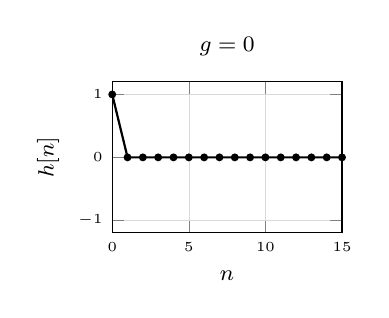
\begin{tikzpicture}
      \begin{axis}[
        width=4.5cm,
        height=3.5cm,
        xlabel={$n$},
        ylabel={$h[n]$},
        xmin=0, xmax=15,
        ymin=-1.2, ymax=1.2,
        grid=major,
        grid style={line width=.1pt, draw=gray!30},
        tick label style={font=\tiny},
        label style={font=\footnotesize},
        title={$g = 0$},
        title style={font=\footnotesize\bfseries}
      ]

      % Risposta con g=0: impulso passa direttamente (feedforward unitario)
      \addplot[
        color=black,
        mark=*,
        mark size=1pt,
        line width=0.8pt
      ] coordinates {
        (0,1) (1,0) (2,0) (3,0) (4,0) (5,0) (6,0) (7,0) (8,0) (9,0) (10,0)
        (11,0) (12,0) (13,0) (14,0) (15,0)
      };

      \end{axis}
    \end{tikzpicture}
    \caption{Passaggio diretto: solo feedforward}
    \label{fig:allpass-zero}
  \end{subfigure}
  \hfill
  \begin{subfigure}[b]{0.32\textwidth}
    \centering
    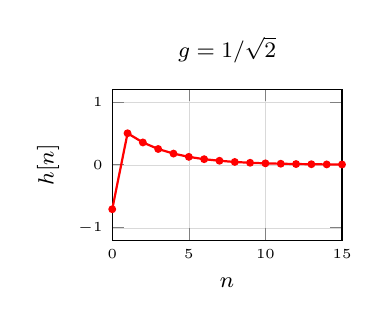
\begin{tikzpicture}
      \begin{axis}[
        width=4.5cm,
        height=3.5cm,
        xlabel={$n$},
        ylabel={$h[n]$},
        xmin=0, xmax=15,
        ymin=-1.2, ymax=1.2,
        grid=major,
        grid style={line width=.1pt, draw=gray!30},
        tick label style={font=\tiny},
        label style={font=\footnotesize},
        title={$g = 1/\sqrt{2}$},
        title style={font=\footnotesize\bfseries}
      ]

      % Risposta AllPass Schroeder corretta con g=1/sqrt(2) ≈ 0.707
      % t=0: -g = -0.707
      % t=τ: (1-g²) = 0.5
      % t=2τ: (1-g²)g = 0.354
      % t=3τ: (1-g²)g² = 0.250
      \addplot[
        color=red,
        mark=*,
        mark size=1pt,
        line width=0.8pt
      ] coordinates {
        (0,-0.707) (1,0.500) (2,0.354) (3,0.250) (4,0.177) (5,0.125)
        (6,0.088) (7,0.063) (8,0.044) (9,0.031) (10,0.022)
        (11,0.016) (12,0.011) (13,0.008) (14,0.005) (15,0.004)
      };

      \end{axis}
    \end{tikzpicture}
    \caption{Equilibrio critico: bilanciamento FIR/IIR}
    \label{fig:allpass-sqrt}
  \end{subfigure}
  \hfill
  \begin{subfigure}[b]{0.32\textwidth}
    \centering
    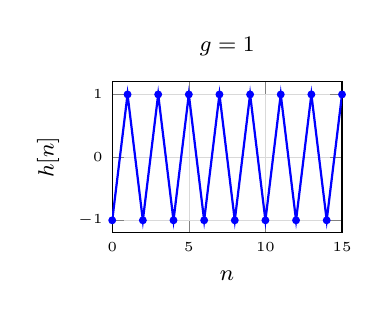
\begin{tikzpicture}
      \begin{axis}[
        width=4.5cm,
        height=3.5cm,
        xlabel={$n$},
        ylabel={$h[n]$},
        xmin=0, xmax=15,
        ymin=-1.2, ymax=1.2,
        grid=major,
        grid style={line width=.1pt, draw=gray!30},
        tick label style={font=\tiny},
        label style={font=\footnotesize},
        title={$g = 1$},
        title style={font=\footnotesize\bfseries}
      ]

      % Risposta AllPass Schroeder con g=1
      % Al limite di stabilità
      \addplot[
        color=blue,
        mark=*,
        mark size=1pt,
        line width=0.8pt
      ] coordinates {
        (0,-1) (1,1) (2,-1) (3,1) (4,-1) (5,1) (6,-1) (7,1)
        (8,-1) (9,1) (10,-1) (11,1) (12,-1) (13,1) (14,-1) (15,1)
      };

      \end{axis}
    \end{tikzpicture}
    \caption{Stallo oscillatorio: dominanza IIR}
    \label{fig:allpass-one}
  \end{subfigure}

% Caption rivisto per i subplot con riferimenti specifici al processo ποίησις
\caption{Dinamiche del processo ποίησις attraverso il filtro AllPass di Schroeder al variare del parametro $g$. ~~~ a) Con $g=0$: la πρᾶξις opera senza memoria teorica, producendo azioni immediate ma prive di risonanza culturale ($H(z) = 1$). ~~~ b) Con $g=1/\sqrt{2} \approx 0.707$: si realizza l'equilibrio creativo aristotelico dove la ποίησις emerge dal bilanciamento dinamico tra πρᾶξις immediata (impulso $-g$ a $t=0$) e θεωρία accumulata (echi decrescenti $(1-g^2)g^n$). ~~~ c) Con $g=1$: la θεωρία domina completamente, il pensiero si cristallizza in pura speculazione senza capacità generativa.}
\label{fig:poiesis-allpass}
\end{figure}


\clearpage

% Nel documento
%\nocite{*}
\printbibliography

\end{document}
